\chapter{ESPECIFICAÇÃO DO PROJETO} % (fold)
\label{cha:especificacao_do_projeto}

 O projeto consiste no desenvolvimento de um sistema de recomendação acoplado a várias redes sociais, sendo que uma dessas redes será desenvolvida neste projeto. Além disso, serão desenvolvidos aplicativos para integração às redes sociais existentes.


\section{Descrição do Sistema}

 Através do sistema os usuários poderão cadastrar produtos e avaliá-los quantitativamente, sendo possível realizar recomendações a outros usuários. Desse modo, o usuário poderá construir a sua reputação. O sistema de recomendação filtra as informações recebidas por todos os usuários, as quais são enviadas por outros usuários, de modo que apenas aquelas relevantes cheguem ao conhecimento das pessoas. As recomendações geradas pelo sistema são baseadas nas opiniões, nas relações sociais entre os usuários e nas relações encontradas entre os produtos. Com base na relação entre usuários, produtos e avaliações o sistema irá inferir as seguintes informações:
\begin{itemize}

 \item Similaridade entre usuários

 \item Similaridade entre produtos

 \item Grau de confiança nas recomendações de um usuário para outro

 \item Grau de reputação global de um usuário baseado nas recomendações diretas

 \item Relação de consumo entre diferentes produtos

 \item Recomendações de produtos mais relevantes para um determinado usuário

\end{itemize}

 Para a obtenção das recomendações será feito um estudo para determinar quais critérios inferidos são mais importantes de forma que o sistema apresente uma boa acurácia, abrangência e alta satisfação dos usuários.

 Ao entrar na rede o usuário tem a opção de buscar produtos já cadastrados e, caso não existam, pode ele mesmo cadastrá-los. Neste cadastro o usuário pode informar a sua opinião referente ao produto e avaliá-lo, possibilitando ao sistema verificar quais são os seus gostos. Com isso, as pessoas podem recomendá-lo para seus amigos presentes na rede social, sendo que essa recomendação deve ser direcionada para as pessoas que o usuário tenha certo conhecimento que gostarão do produto.

 Os usuários que recebem a recomendação podem acessar o cadastro do produto e avaliá-lo para que o sistema atualize as informações relativas aos seus gostos. Estas informações são utilizadas para verificar a similaridade entre usuários, ou seja, usuários que tenham gostos semelhantes. A avaliação altera o grau de confiança entre o usuário que recomendou o produto e o que recebeu. Caso a avaliação tenha um grau positivo, a confiança do receptor aumenta, porém, caso a avaliação tenha um grau negativo, significa que o usuário que recebeu a recomendação não a aceitou como relevante, fazendo com que o grau de confiança no outro usuário diminua.

 O sistema armazena todas essas informações referentes à avaliação de produtos e de confiança entre usuários para filtrar recomendações entre usuários com baixo grau de confiança. Esse é um dos propósitos do sistema de recomendação: mostrar à pessoa apenas informações relevantes. Ou seja, caso a pessoa receba recomendações sem conteúdo plausível de um usuário, seu grau de confiança diminui e, quando esta diminuir até um limite, o sistema passa a não mostrar mais recomendações desse usuário.

 Também é função do sistema de recomendação realizar recomendações aos usuários para incentivar a avaliação de produtos, pois é assim que as pessoas fornecem informações referentes aos seus gostos. Tais recomendações são relativas aos produtos mais bem avaliados na rede e também aqueles bem avaliados por amigos com alto grau de confiança.

\begin{figure}
  \centering
  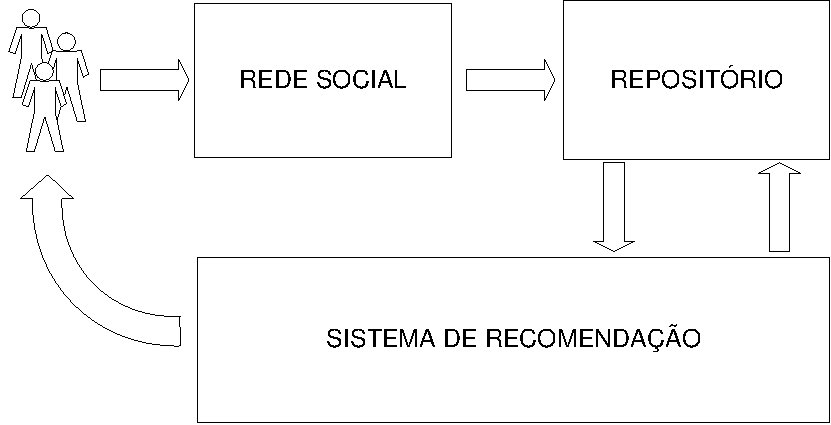
\includegraphics[width=\textwidth]{imagens/Diagrama_Visao_Geral}
  \caption{\it Diagrama de blocos do sistema}
  \label{fig:escopo}
\end{figure}

A Figura~\ref{fig:escopo} exibe o diagrama de blocos do sistema.


\section{Funcionalidades principais} % (fold)
\label{sec:funcionalidades_principais}

Abaixo estão sumarizadas as principais funcionalidades do sistema:

\begin{itemize}

	\item Recomendação de produtos baseada em preferência do usuário
	\subitem Como usuário, eu quero receber uma lista de produtos que eu provavelemente goste para que eu não precise filtrar os itens que me interessam.

	\item Permitir que o usuário avalie um produto
  \subitem Como usuário, quero fazer a minha avaliação de produtos para que outros tenham conhecimento da minha opinião.

	\item Permitir que o usuário envie uma recomendação a outro usuário
  \subitem Como recomendador, quero enviar uma recomendação de produto para outra pessoa para que ela conheça a minha opinião sobre este item.

	\item Exposição das avaliações em formatos abertos
  \subitem Como agente web, quero obter as avaliações dos usuários em formato padronizado (e aberto) para que possa interpretar estas avaliações.

    \item Cadastro de novos produtos
    \subitem Como usuário, quero poder cadastrar um novo produto que ainda não está cadastrado.
    
    \item Importação de conteúdo em formato aberto
    \subitem Como usuário, quero poder informar uma fonte de conteúdo em formato aberto para que possa adicionar dados externos ao repositório.

    \item Explicação automática ao usuário do porquê daquele item ter sido recomendado
    \subitem Como usuário, quero obter a explicação sobre as recomendações recebidas para analisar criticamente a recomendação e me motivar a avaliar o produto.

    \item Visualização das avaliações recentes dos amigos
    \subitem Como usuário, quero estar ciente sobre as últimas avaliações dos meus amigos para que eu possa saber o que acontece no meu contexto social e conheça novos produtos.

    \item Feedback de recomendação
    \subitem Como recomendador, quero receber feedback sobre as recomendações que enviei para me incentivar a fazer melhores recomendações.

	
\end{itemize}

\section{Requisitos não-funcionais}

Os principais requisitos não-funcionais do sistema são:

\begin{itemize}

    \item Interface web compatível as últimas versões dos \textit{browsers} Internet Explorer, Mozilla Firefox e Safari.
    
    \item \textit{Backend} compatível com servidores Linux.

    \item Tempo médio de resposta menor que 2 segundos para 10 usuários simultâneos quando executado em um servidor com processador Intel Core 2 Duo T7250 ou superior e 2 GB de memória RAM. % esta é a configuração do meu notebook -- Allan

\end{itemize}

\section{Limites do Sistema}

\begin{itemize}
  
    \item O sistema não fará processamento de linguagem natural\footnote{\textit{Natural Language Processing (NLP)}}

\end{itemize}

\section{Tecnologia} % (fold)
\label{sec:tecnologia}

% section tecnologia (end)

\section{Planejamento e Métodos} % (fold)
\label{sec:planejamento_e_métodos}


% section planejamento_e_métodos (end)

% chapter especificacao_do_projeto (end)
